% Chapter 6

\chapter{Results and Discussion} % Main chapter title

\label{Chapter6} % For referencing the chapter elsewhere, use \ref{Chapter6} 

\lhead{Chapter 6. \emph{Results and Discussion}} % This is for the header on each page - perhaps a shortened title

%----------------------------------------------------------------------------------------

%ques: do we need a reference here to the enron dataset?

\section{Introduction} %ques: TODO
In chapter 5, Software Design Description (SDD) was explained. System architecture, main components and their functionalities, as well as components interaction were discussed. In this chapter, experiments of different classification proceduers, dataset splits and feature selection are presented. Results are introduced in section 6.2. The discussion and analysis of obtained results are presented in section 6.3.


\section{Experimental Setup}
We report two types of experiments:

\begin{itemize}
\item Learning Curves (Timeline): We calculate the accuracy for each training/test split and plot the classification accuracy curve over the number of training messages in the splits. %ques: we need a reference to the paper here?

\item Feature Comparison: We select different combinations of possible classification features and plot the accuracy of each combination
Selecting several email features and calculating the classification accuracy for each selection. 
\end{itemize}

\subsection{Training/test Set Splits}
In practice, the dataset grows over time. So, a natural way of splitting the dataset would be based on time: train on earlier emails and test on later ones. A similar approach is employed in (Klimt and Yang, 2004). %{add ref here}
The incremental time-based split is done by sorting the emails according to their time stamp, then the classifier is trained on the first N messages and tested against the following N messages, then it is trained on the first 2N messages and tested against the following N messages etc. until we cover the whole dataset. N was chosen to be 100 which is similar to experiments conducted in (Bekkerman, McCallum and Huang 2004)

\section{Results}

\subsection{Learning Curves}
Results of the seven Enron users are presented below as the accuracy over the timeline of each user.

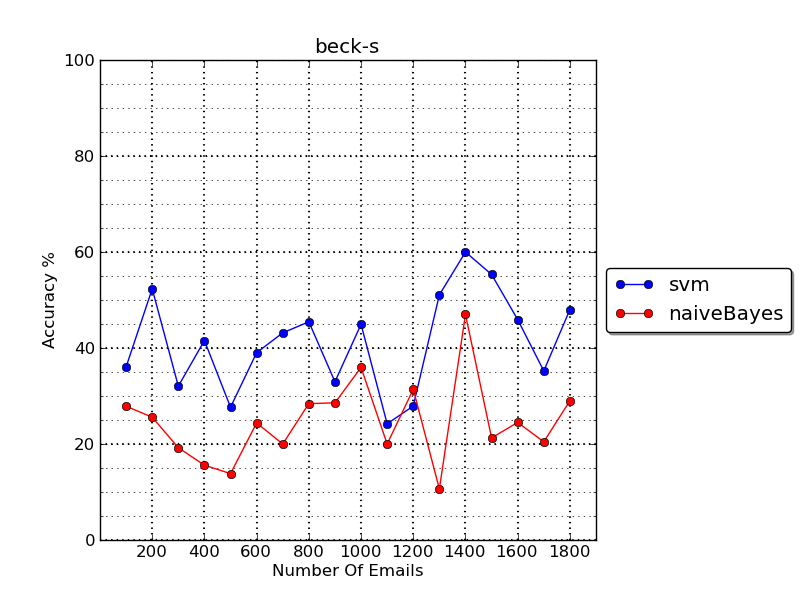
\includegraphics[width=15cm]{beck-s.png}
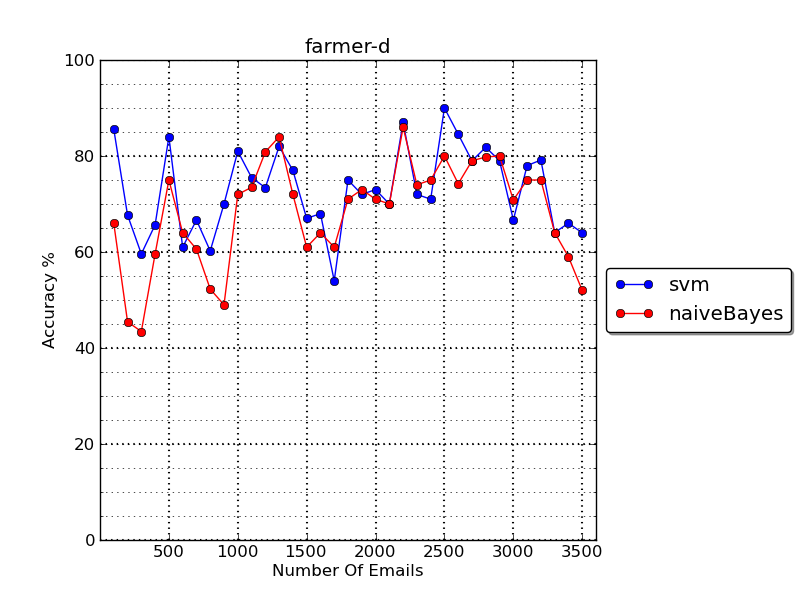
\includegraphics[width=15cm]{farmer-d.png}
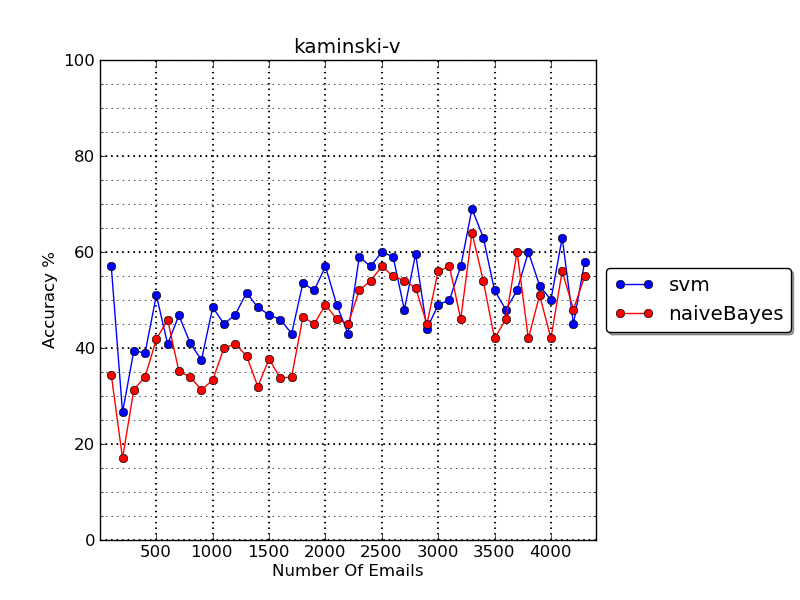
\includegraphics[width=15cm]{kaminski-v.png}
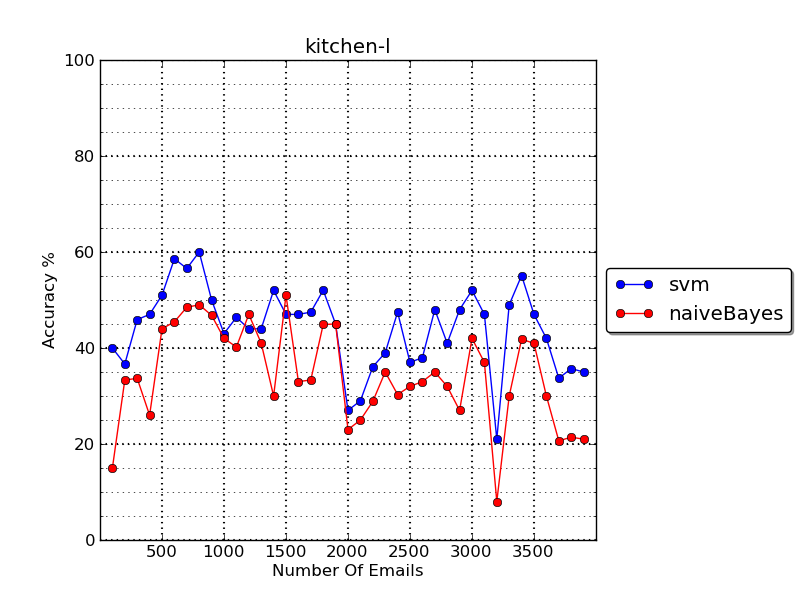
\includegraphics[width=15cm]{kitchen-l.png}
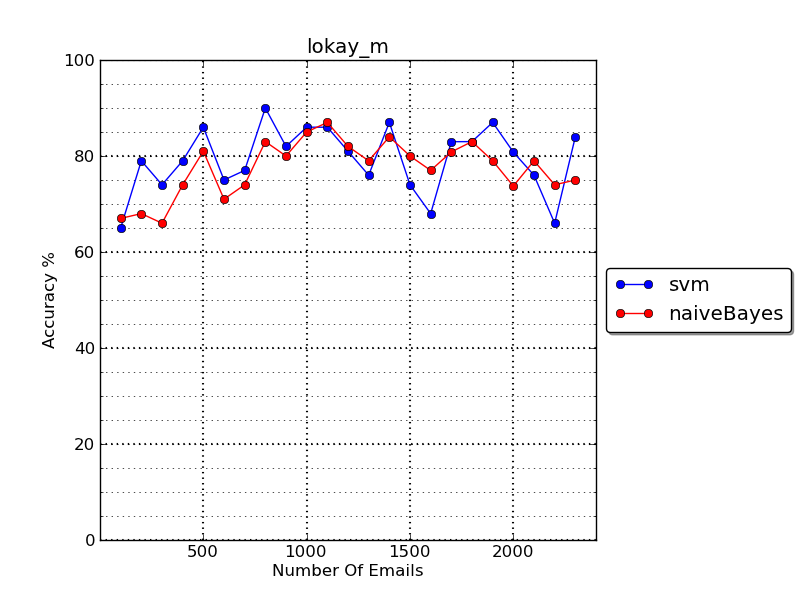
\includegraphics[width=15cm]{lokay_m.png}
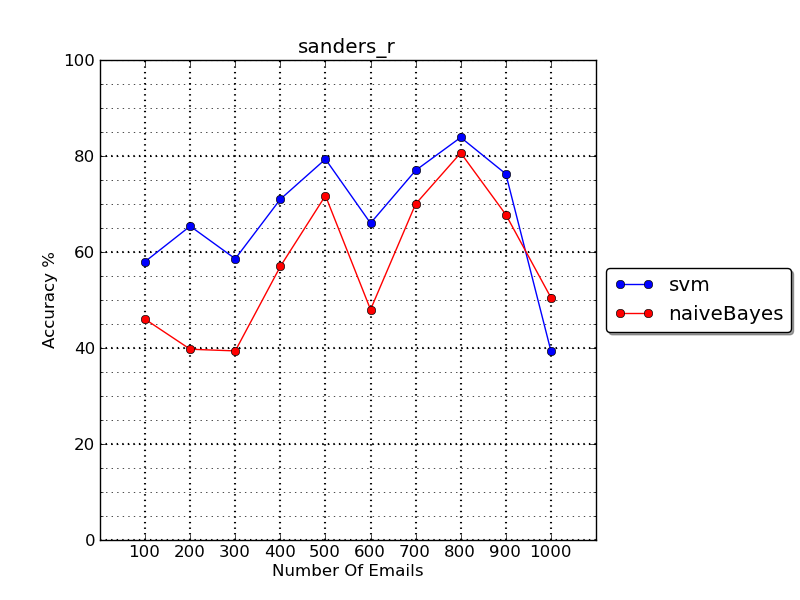
\includegraphics[width=15cm]{sanders_r.png}
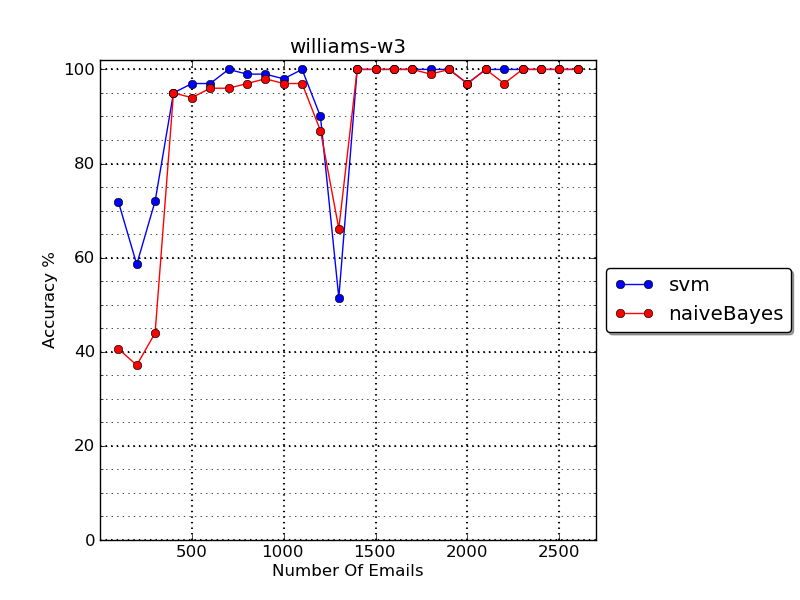
\includegraphics[width=15cm]{williams-w3.png}

The following table is the accuracies averaged over all training/test splits for all users. It has two columns representing the 2 different classification algorithms: Naive Bayes and SVM.

\begin{center}
    \begin{tabular}{ | l | l | l |}
    \hline
    User {\textbackslash}  Classifier & Naive Bayes & SVM \\ \hline
    Beck-s & 24.65\% & 41.27\% \\ \hline
    Farmer-d & 68.36\% & 72.87\% \\ \hline
    Kamniski-v & 44.53\% & 50.36\% \\ \hline
    Kitchen-l & 34.44\% & 44.15\% \\ \hline
    Lokay\_m & 77.50\% & 79.34\% \\ \hline
    Sanders\_r & 57.08\% & 67.49\% \\ \hline
    Williams-w3 & 89.92\% & 93.30\% \\
    \hline
    \end{tabular}
\end{center}

\subsection{Feature Comparison}
In classification, different combinations of the features affect accuracy. It is not necessarily that adding a feature will improve accuracy. So, it was important to test different features combinations to select the best combination. The results for six different combinations are reported below for each user. Each combination is tested under both Naive Bayes and SVM classification algorithms.

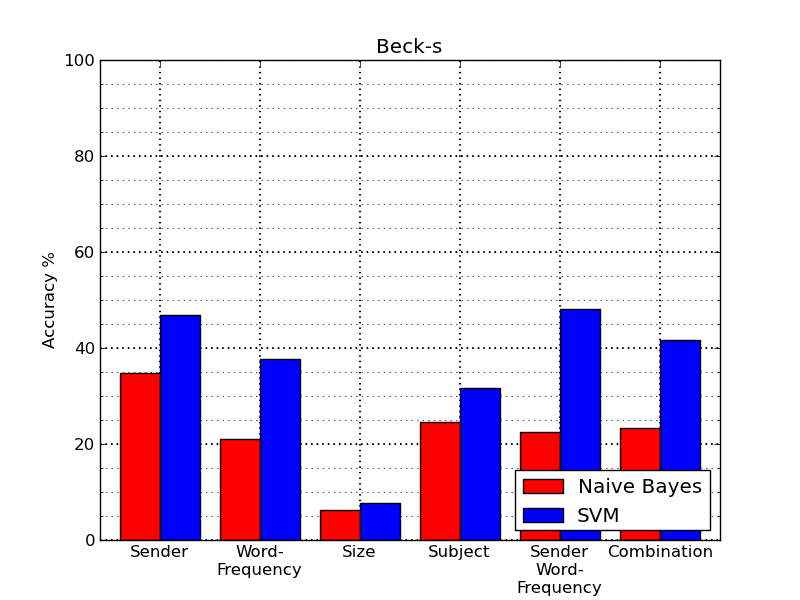
\includegraphics[width=15cm]{F_Beck-s.png}
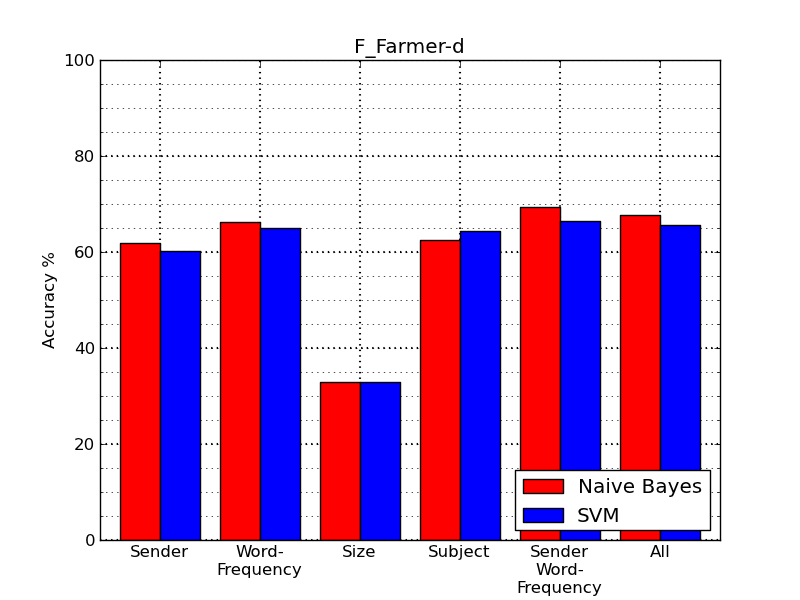
\includegraphics[width=15cm]{F_Farmer-d.png}
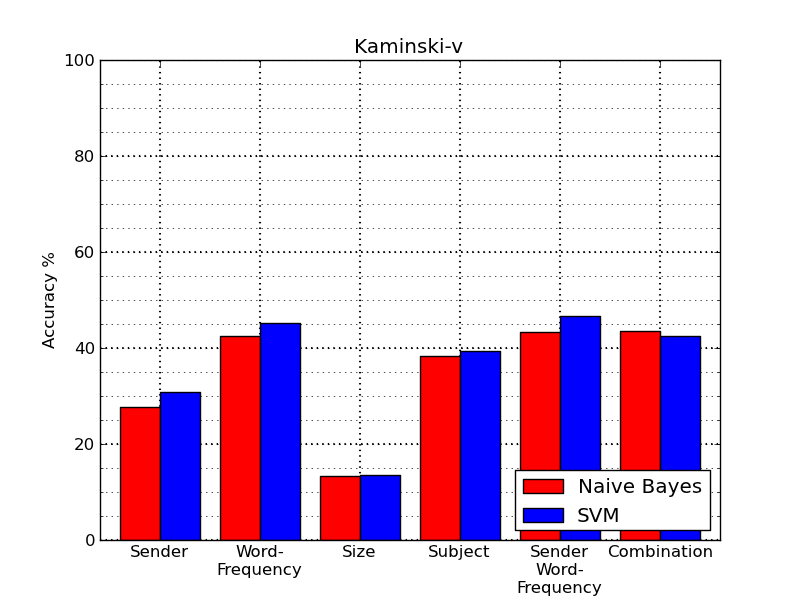
\includegraphics[width=15cm]{F_Kaminski-v.png}
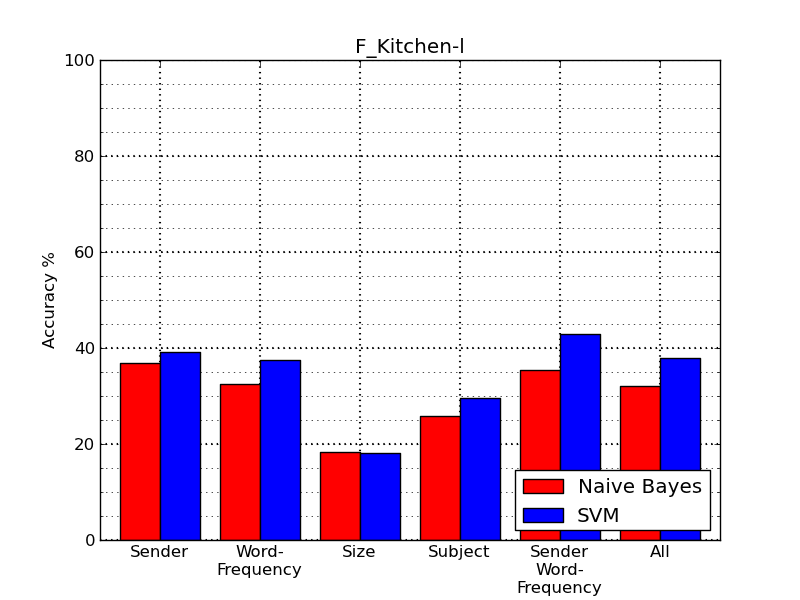
\includegraphics[width=15cm]{F_Kitchen-l.png}
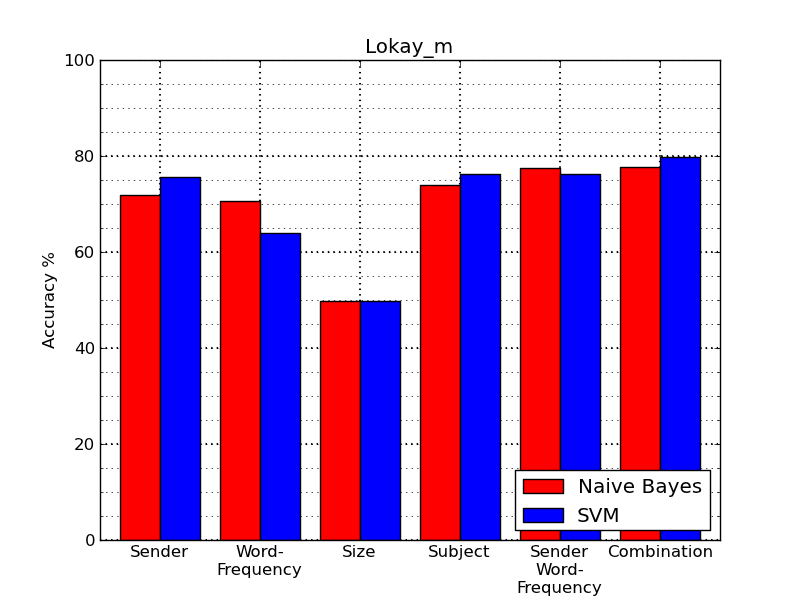
\includegraphics[width=15cm]{F_Lokay_m.png}
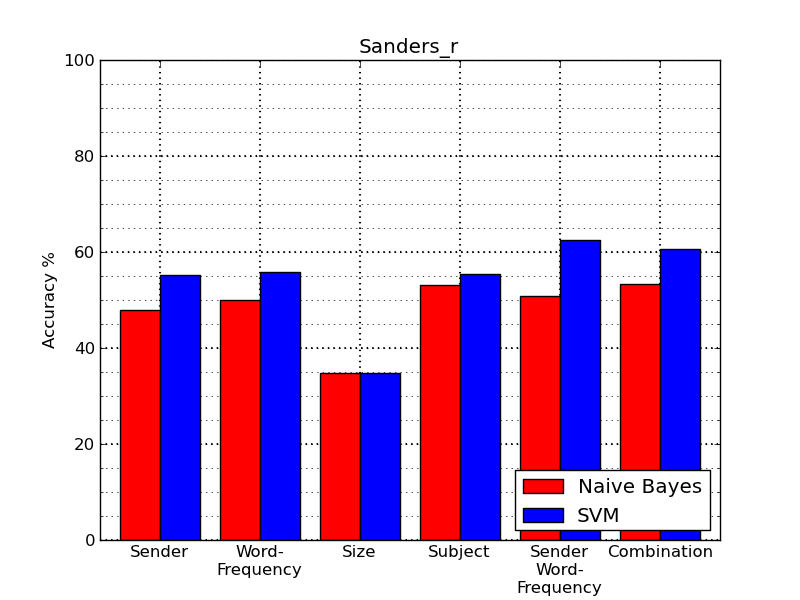
\includegraphics[width=15cm]{F_Sanders_r.png}
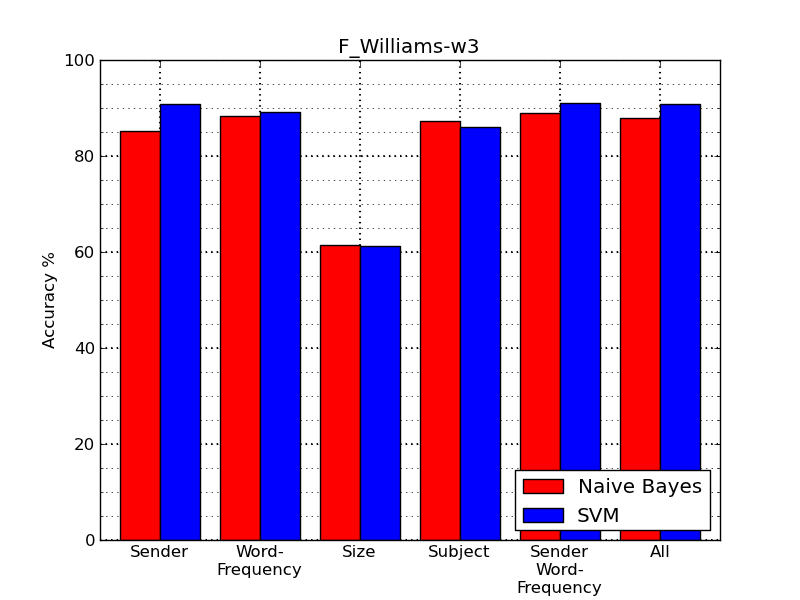
\includegraphics[width=15cm]{F_Williams-w3.png}

\section{Discussion}
Learning curves show that SVM outperforms Naive Bayes in most of the cases. This is the expected behaviour. It is widely believed that Naive Bayes is not the best algorithm for text categorization (Dumais et al., 1998). %add ref. here
However, the results obtained doesn't reveal significance superiority of SVM over Naive Bayes. In fact, in some cases Naive Bayes was better than SVM (e.g Farmer-d feature selection figure). This is probably due to features selection and how the classifier weights each feature.


Experimental results obtained support the following observations:
\begin{itemize}
\item Accuracies are higher when the dataset has one or two dominant folders. As it can be seen from Tables X,%add table!
 the size of the largest folder is nearly one half size of the entire dataset(e.g., users lokay\_m and williams-w3).

\item Newly created folders negatively affects the classification accuracy. If a new folder is created, the classifier trains on few emails from this folder which may not be enough to build a good classification model. (e.g see the drops in sanders\_r and william-w3 learning curves)

\item The dataset of user williams-w3 is a degenerative case. It has two large folders ("bill williams iii" and "schedule crawler" which contain most of the messages. This explains the high accuracy for this dataset regardless of the features used.
\end{itemize}

In this chapter the experimental results were presented. Analysis of the results were discussed. The results reveal the difficulty of eamil classification. Improving the accuracy is listed as a future work.

